\section{Ejercicio 6 - Round Robin vs FCFS}

Se ejecutó una simulación con el mismo lote utilizado en la sección 5, pero esta vez con un Scheduler FCFS.  La Figura \ref{fig-ej6} muestra el gráfico de dicha simulación. Los promedios de latencia, waiting-time y tiempo total de ejecución se muestran en el Cuadro \ref{tab-promedios}.

\begin{figure}[!htb]
\begin{center}
  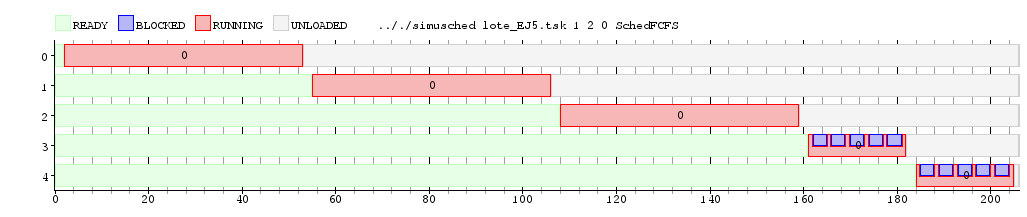
\includegraphics[scale=0.45]{imagenes/ej6.png}
\end{center}
\caption{Simulación para FCFS, 1 núcleo y 2 ciclos de cs}\label{fig-ej6}
\end{figure}

\begin{table}[!htb]
\begin{center}
\begin{tabular}{| l | l | l | l | l |}
\hline
Scheduler & Quantum & Latecia & Waiting-time & Total ejecución\\
\hline
RR & 2 & 9.8 & 208.8 & 247.8\\
\hline
RR & 10 & 24.2 & 180 & 219\\
\hline
RR & 50 & 96.2 & 141.6 & 180.6\\
\hline
FCFS & - & 102 & 102 & 141\\
\hline
\end{tabular}
\end{center}
\caption{Promedios - SchedRR y FCFS}\label{tab-promedios}
\end{table}

Podemos observar en la tabla de promedios del Cuadro \ref{tab-promedios}, que la latencia del FCFS es muy parecida a la del Round Robin con quantum 50, pero los valores de waiting-time y tiempo total de ejecución son significativamente menores. Considerando los resultados obtenidos en el ejercicio 5, podríamos concluir que de tener poca importancia, en cierto contexto de uso, el tiempo que una tarea tarda en empezar a ejecutar, utilizar FCFS tiene una mejor utilización de los recursos del cpu, dejándolo desocupado el menor tiempo posible (con las opciones con las cuales disponemos). Sin embargo, de ser prioritario el tiempo de respuesta de una tarea, sigue siendo más conveniente usar Round Robin con quantum 2.